\subsection{Systembeschreibung}
Die Umsetzung der Wissenserwerbskomponente erfolgt am Beispiel vom \textit{PaaSfinder}\footnote{{\label{foot:paasfinder}}https://paasfinder.org}, einem Expertensystem und Open-Source-Projekt im Bereich von \acf{PaaS}. Das Ziel des Systems besteht darin, zahlreiche PaaS-Anbieter vergleichbar zu machen. \textit{PaaSfinder} verf�gt bereits �ber eine Wissensdatenbank, die PaaS-Profile beinhaltet und aufgrund der h�ufigen �nderungen im gegebenen Anwendungsbereich regelm��ig aktualisiert werden muss. Die Struktur von \textit{PaaSfinder} l�sst sich in der Abbildung \ref{fig:paasfinder} folgenderma�en beschreiben.
\begin{figure}[H] 
	\centering
	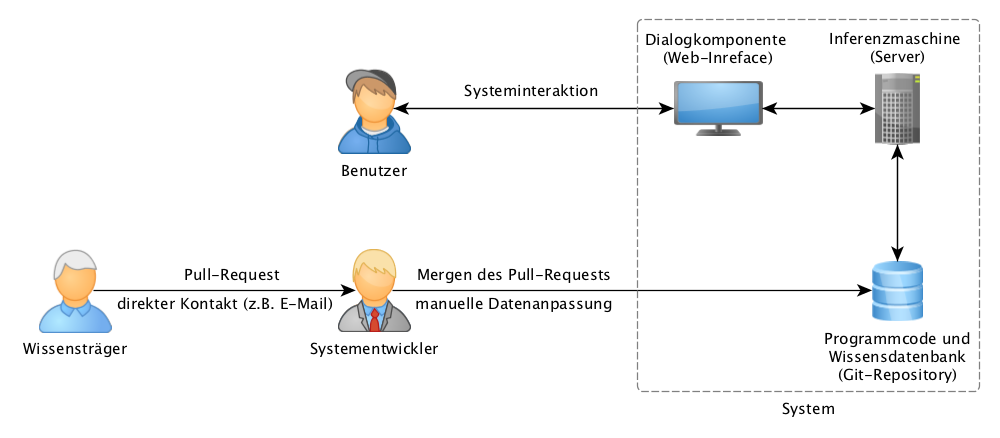
\includegraphics[width=1.0\textwidth]{images/paasfinder.png}
	\caption{Die Struktur vom \textit{PaaSfinder}}
	\label{fig:paasfinder}
\end{figure} 
\textit{PaaSfinder} setzt sich aus dem Programmcode mit der Wissensdatenbank und der Webanwendung zusammen. Die Webanwendung wird wiederum auf einem Server betrieben. Ein PaaS-Anbieter wird in einem Profil\footnote{https://github.com/stefan-kolb/paas-profiles\#profile-specification} beschrieben, das wie folgt aufgebaut ist:
\begin{enumerate}
\item \textbf{General Properties}: allgemeine Eingenschaften des PaaS-Anbieters (z.B. Name, URL, Status, Type, etc.)
\item \textbf{Extensible}: generelle Erweiterungsm�glichkeit nach Kundenbedarf (z.B. spezielle Laufzeitumgebung)
\item \textbf{Pricing}: verf�gbare Preismodelle
\item \textbf{Quality of Service}: die Servicequalit�t (z.B. Verf�gbarkeit)
\item \textbf{Hosting}: Art der Bereitstellung (z.B. privat)
\item \textbf{Scaling}: Skalierbarkeit (z.B. Speichererweiterung)
\item \textbf{Runtimes}: unterst�tzte Laufzeitumgebungen (z.B. Java\footnote{https://java.com})
\item \textbf{Middleware} (z.B. Tomcat\footnote{https://tomcat.apache.org})
\item \textbf{Frameworks} (z.B. Play\footnote{https://www.playframework.com})
\item \textbf{Services} (z.B. Datenspeicher)
\item \textbf{Infrastructures} (z.B. Informationen zum Standort)
\end{enumerate}
Ein Profil wird als ein \acs{JSON}\footnote{\label{foot:json}http://json.org}-Eintrag gespeichert. JSON stellt ein Datenaustauschformat dar und basiert auf zwei Datenstrukturen: 
\begin{itemize}
\item \textit{Name/Wert Paar}, das als ein Objekt darstellt (siehe Abbildung \ref{fig:json-object}).
\item \textit{Eine geordnete Liste von Werten (Array)}, die kein oder mehrere durch Komma getrennte Objekte enth�lt (siehe Abbildung \ref{fig:json-array}).
\end{itemize}
\begin{figure}[H] 
	\centering
	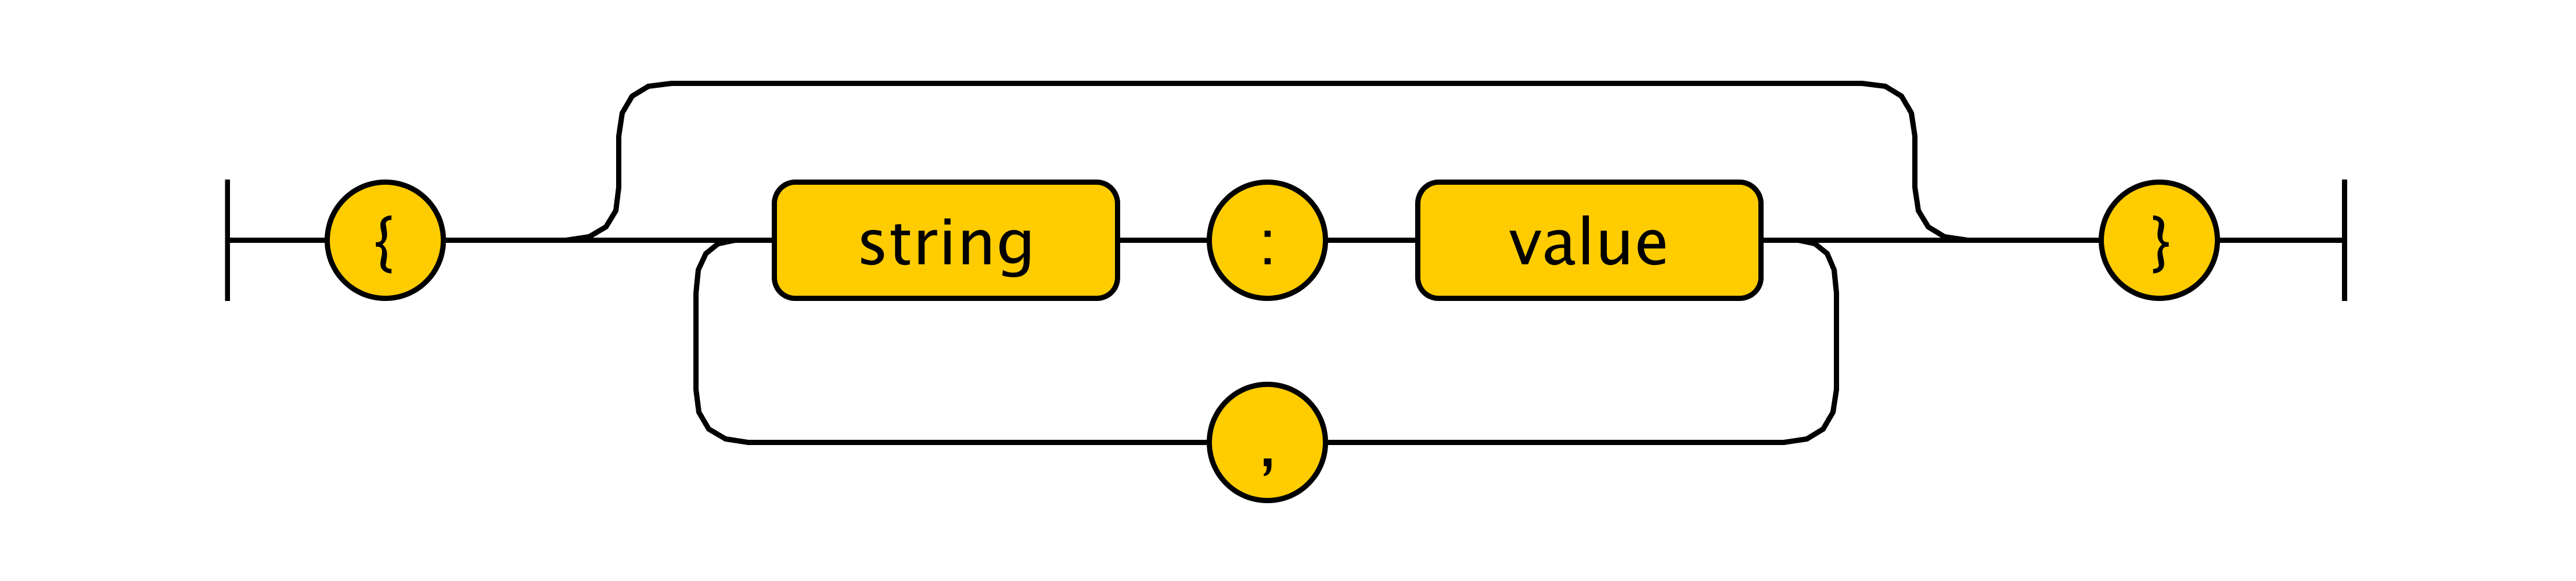
\includegraphics[width=1.0\textwidth]{images/json-object.png}
	\caption{JSON-Objekt Spezifikation, \ref{foot:json}}
	\label{fig:json-object}
\end{figure} 
\begin{figure}[H] 
	\centering
	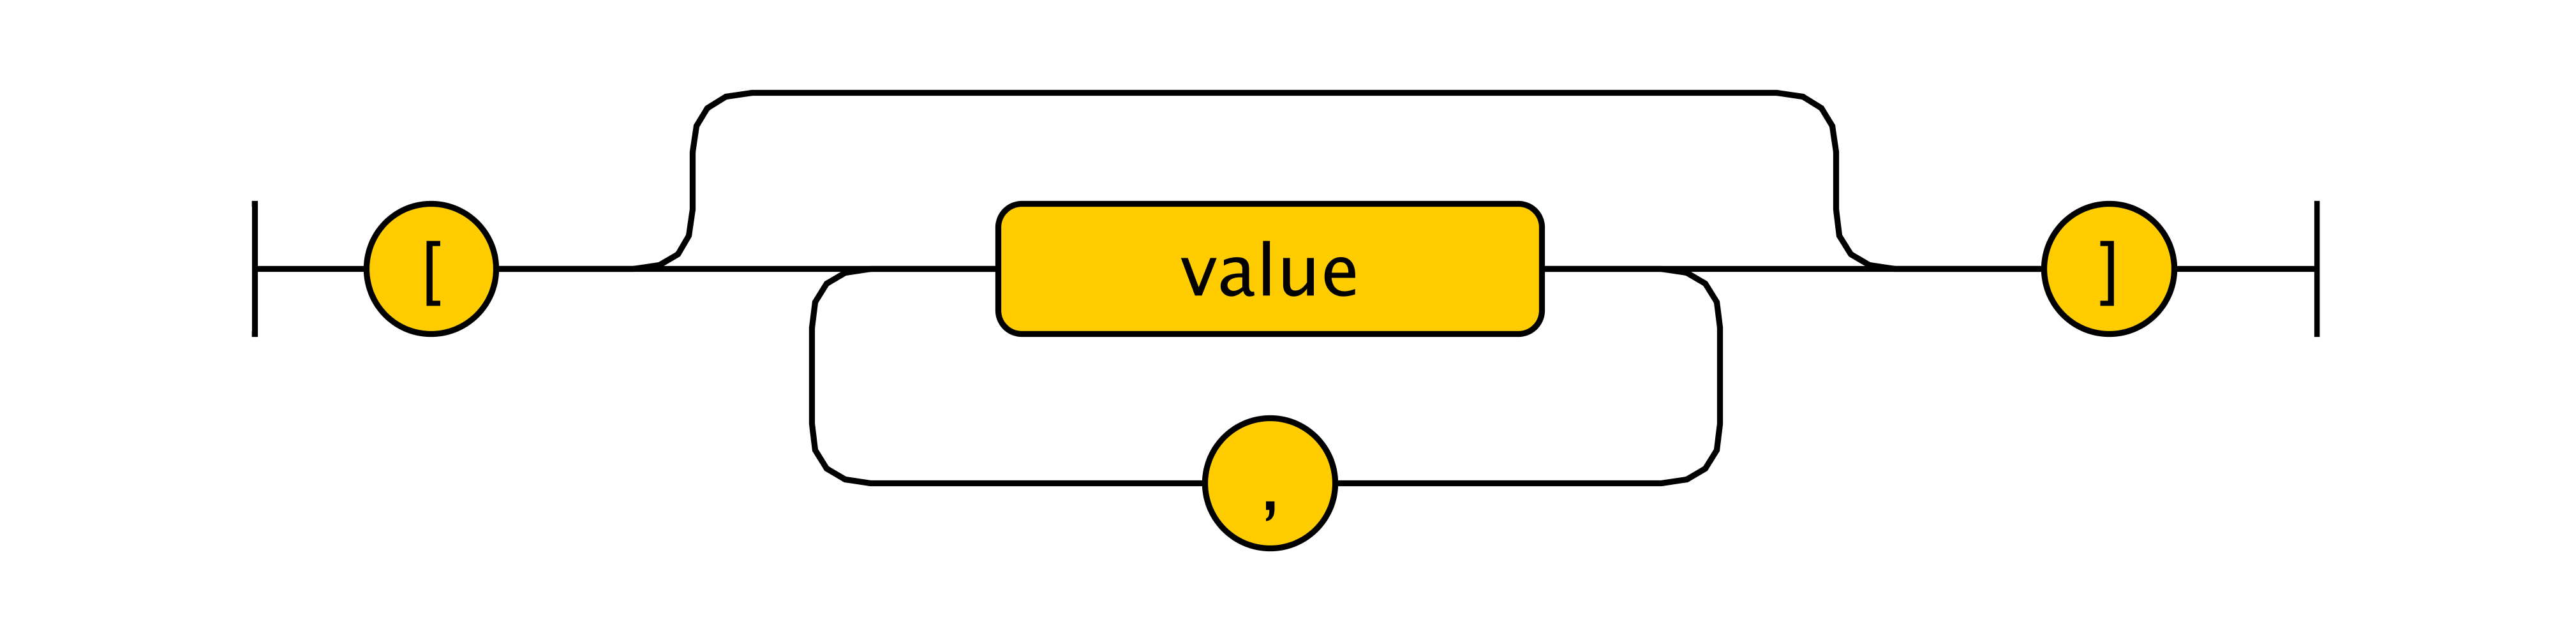
\includegraphics[width=0.9\textwidth]{images/json-array.png}
	\caption{JSON-Array Spezifikation, \ref{foot:json}}
	\label{fig:json-array}
\end{figure} 
Die Wissensdatenbank und der Programmcode von \textit{PaaSfinder} befinden sich in einem Git-Repository. Bei Git\footnote{https://git-scm.com} handelt es sich um ein verteiltes System zur Projektverwaltung. Da \textit{PaaSfinder} ein Open-Source-Projekt ist, kann jeder der Wissensdatenbank beitragen. Momentan kann das auf zwei Weisen erfolgen (siehe Abbildung \ref{fig:paasfinder}):
\begin{itemize}
\item \textit{Pull-Request\footnote{https://git-scm.com/docs/git-request-pull}}
\item \textit{Direkter Kontakt mit dem Systementwickler} 
\end{itemize}
Beim Pull-Request wird das gesamte Projekt-Repository lokal gespeichert. Danach werden �nderungen vorgenommen und anschlie�end einen Pull-Request erstellt. Der Pull-Request wird vom Projektmaster �berpr�ft und zugeh�rige �nderungen �bernommen (\glqq{}gemerged\grqq{}), falls keine Konflikte vorliegen. Wenn der Wissenstr�ger mit dem Git-System nicht vertraut ist, kann ein direkter Kontakt (beispielsweise per E-Mail) mit dem Systementwickler aufgenommen werden. Die Daten werden dann manuell vom Systemverwalter in die Wissensbasis eingetragen.\\
Sowohl Pull-Request als auch Kontakt mit dem Systementwickler entspricht dem direkten Wissenserwerb gem�� der Klassifikation in Kapitel \ref{subsec:Wissenserwerbskomponente}. Der Vorteil dabei ist, dass die Daten nicht manuell gesucht werden sollen, sondern gleich vom Wissenstr�ger stammen. Anderseits wird die Datenerfassung durch Git-Kenntnisse des Wissenstr�gers beschr�nkt. Um den direkten Wissenserwerb zu erleichtern, wird im weiteren Verlauf die Wissenstr�gerschnittstelle entwickelt, die es dem Wissenstr�ger erm�glicht, einen bestehenden PaaS-Eintrag zu aktualisieren. Nach dem erfolgreichen Absenden der �nderungen soll automatisch ein Pull-Request erstellt werden. 